\documentclass[a4paper, 12pt, titlepage, oneside, french]{article}

\usepackage[francais]{babel}
\usepackage[utf8]{inputenc}
\usepackage{fancyhdr}
\usepackage{graphicx}
\usepackage{amsmath}
\usepackage{amssymb}
\usepackage[backend=biber,sorting=none]{biblatex}
\usepackage{float}
\usepackage{subcaption}
\usepackage{hyperref}
\usepackage{spverbatim}
\usepackage[margin=1.2in]{geometry}

\graphicspath{ {images/}}
\addbibresource{Biblio.bib}

\author{Martin Olivier, Fabien Goglio}
\title{Rapport InSite}

\pagestyle{fancy}

%Put the chapter and section header in lowercase
%\renewcommand{\chaptername}[1]{%
%	\markboth{#1}{}}

\renewcommand{\sectionmark}[1]{%
	\markright{\thesection\ #1}}

\fancyhf{}
%\fancyhead[LE, RO]{\bfseries}
\fancyhead[LO]{\bfseries\textit\rightmark}
%\fancyhead[RE]{\bfseries\textit}
\fancyhead[RE]{WAT}
\renewcommand{\footrulewidth}{0.5pt} %space for the rule
\fancypagestyle{plain}{\fancyhead{}, %get rid of header on plain pages
	\renewcommand{\headrulewidth}{0pt} % and the line
}
\fancyfoot[L]{2017 -- 2018}
\fancyfoot[R]{Page \thepage}

\begin{document}
\begin{titlepage}
	\centering
		\vfill
		    {\bfseries\Large
			Rapport de Mi-Parcours\\
			InSite\\
			Janvier 2018\\
			\vskip2cm
			Martin OLIVIER, Fabien GOGLIO\\
		    }    
		\vfill
		
\includegraphics[width=8cm]{Logo_Preview.png}
		\begin{figure}[b]
			
\includegraphics[width=4cm]{Logo-ESIEA.jpg}

		\end{figure}
		\vfill
		\hfill {\bfseries\Large
		 Suiveur:\\
		 \hfill Sylvie ZAGO}
\end{titlepage}

\pagenumbering{roman}
\newpage
	\tableofcontents
\newpage
\cleardoublepage
\pagenumbering{arabic}
\section{Remerciement}
	Nous tenons a remercier \[...\]
	\newpage
\section{Introduction}
	Dans ce rapport nous présentons l'avancement de notre Projet Scientifique et Technique de troisième année.
	Vous trouverez dans ce document le descriptif de notre projet, ses objectifs ainsi que toute notre démarche de gestion de projet.

	\paragraph{}

	Étant donnée que notre projet conduit principalement un travail de recherche, sur les conseils de notre suiveur, nous avons choisi de vous présenter l'avancement de notre travail et le premiers résultats que nous obtenons. \\
	Ainsi, ce rapport décrit aussi notre démarche scientifique : notre approche initiale du problème, les résultats obtenus et les pistes de recherches pour le futur qui en découlent.
	
	\newpage
\section{Présentation}
	\subsection{Description}%Enoncer clairement la problematique et mieux decrire le projet
		InSite analyse et détecte des objets archéologiques dans des relevés géomagnétiques, en utilisant des techniques novatrices dans le domaine de
		la Computer Vision, ainsi que de l'apprentissage automatique.
	\subsection{Objectifs}%Il faut hierarchiser les objectifs et les replacer dans le contexte + SMART
	Nous cherchons a:
	\begin{itemize}
		\item Analyser automatiquement des relevés géomagnétiques 
		\item Produire des cartes d'intérêts, en indiquant les zones ou des objets archéologiques pourrait se trouver
		\item Détecter et réduire le bruit présent dans l'image
	\end{itemize}

	\newpage

\section{Cadrage}
	\subsection{Budget}
	Étant d'abord et surtout un projet de recherche d'informatique, InSite ne requiert pas de budget. Nous avons pu obtenir les relevés magnéto-métrique sans coût, et les ressources nécessaires pour mener à bien ce projet sont déjà à notre disposition. 
	\subsection{Organisation}
	InSite se compose de 2 étudiants, Fabien GOGLIO et Martin OLIVIER. Par cette taille réduite, l'organisation est simplifiée. Les rôles sont distribue selon l'intérêt de pour la tache, et selon sa compétence a mener cette tache a bien. Les recherches sur les techniques a utiliser, et le développement d'outil et de code sont faites de manières indépendantes, même si une communication constante est faite. 
	\subsubsection{Démarche}
	Comme inSite est un projet non pas de développement, mais de recherche, nous utilisons une démarche différentes de celle trouve habituellement dans les PST: nous passons une grande partie de notre temps a faire des recherches, et nous n'écrivons que des petits scripts, qui répondent a une tache particulière. Par exemple, l'application de l'algorithme de Canny, pour la détection de bords sur les relevés,
	ou le découpage des cartes en carres pour l'analyse. Quelques exemples sont disponibles en Annexe %Rajouter canny.py et CutImage.py en annexe
	\subsection{Planning}
	\subsubsection{Dates Clefs}
	\subsection{Langages et technologies utilisées}
	Pour simplifier le développement, nous utilisons Python2 avec les librairies numpy, pyplot, cv2, qui possèdent de nombreuse fonctions mathématique et d'analyse d'image déjà implémentées.
	\newpage

\section{Démarche Initiale}
	
	\subsection{Relevés géomagnétiques et origine de notre dataset}
	Les relevés géomagnétiques sont utilise en archéologie depuis une vingtaine d'années. Ils permettent notamment d'obtenir une idée de la répartition d'objets et structures archéologiques. Un tel relevé s'obtient en mesurant le magnétisme du sol, grâce a un gradiomètre magnétique, qui mesure la différence entre deux mesures du champs magnétiques faites par deux capteurs.
	%Schema + Explication du principe
	On construit ensuite des cartes en noir et blanc, représentant les variations du champs magnétique par une variation de niveau de gris. Une valeur positive forte sera blanche, tandis qu'une valeur négative forte sera noire. Ces relevés permettent de détecter des structures et objet enfouis jusqu'à quelques mètres de profondeur. En effet lorsque l'on construit, ou lorsque l'on fait cuire a l'aide de fours, on modifie les valeurs de champs magnétiques du terrain, et ces variations peuvent être observe. Ces relevés, mesurant le magnétisées du sol sont également très sensible aux objets métalliques, et le sont d'autant plus que ces objets sont proche du capteur, ce qui peux poser problèmes dans les zones ou une activité anthropologique récente a une lieu, car l'homme moderne rejette beaucoup de déchet métalliques. Ces objets métalliques contemporains sont des dipôles et provoquent sur les relevés des anomalies très caractéristiques. Nous discuterons de ces anomalies plus bas.

	Nos relevés nous proviennent tous du site archéologique de Marsal, en Moselle, et ont été réalisés au cours d'une quinzaine d'année, lors de la campagne de fouille de Laurent OLIVIER.%TODO: CONTEXTUALISER%
	. Cette région possède des marais salants, et on trouve des traces d'une exploitation industrielle très importante aux alentours de l'age du Fer (VII\textsuperscript{ème}-I\textsuperscript{ème} siècle avant J.C). On trouve des traces de ces exploitations avec par exemple une quantité extrêmement élevée de briquetage (déchets de terre cuite, utilise pour la cuisson de la saumure); ce n'est pas moins de 4 millions de mètres cube de briquetage accumule dans la région, soit presque deux fois le volume de la pyramide de Kheops. Le sel était, et a longtemps été une ressource stratégique; car en plus de servir d'épice, le sel est utilise dans la conservation d'aliments, et les populations agricultrice, qui consomme moins de viande doivent supplémenter leur apport par du sel. La région a donc été très riche par le passe. Dans les fouilles, on trouve nombre de fours de grande taille, en forme de "U", qui servaient a la préparation du sel, et les corps trouves sur les sites de productions de sel sont mal nourris, ce qui semble indiquer que ce sont des esclaves, ou en tout cas des "employés" qui ne possèdent pas les fours ni le sel qu'ils produisent. %Donner source plus exemples de releves 

	\newpage
	\subsection{Détections d'objets}
	Nous avons décidé de débuter nos recherches de détections de formes par des solutions simples, avec l'attente qu'elle nous donnent des résultats de bonne qualité. L'attrait de ces méthodes étaient principalement qu'elles ne requiert pas de quantité de données importante, et qu'elles étaient a notre porte d'un point de vue académique. Nous avons donc approche le problème de deux façons différentes:
	\begin{itemize}
		\item Filtrage
		\item Algorithmes de détections de bords.
	\end{itemize}
	\subsubsection{Filtrage}
	Nous avons cherché à "nettoyer" les images : atténuer le bruit, très présent dans certaines zones de l'image, et assez handicapant pour la détection de bord.
	\begin{figure}[H]
		\centering
		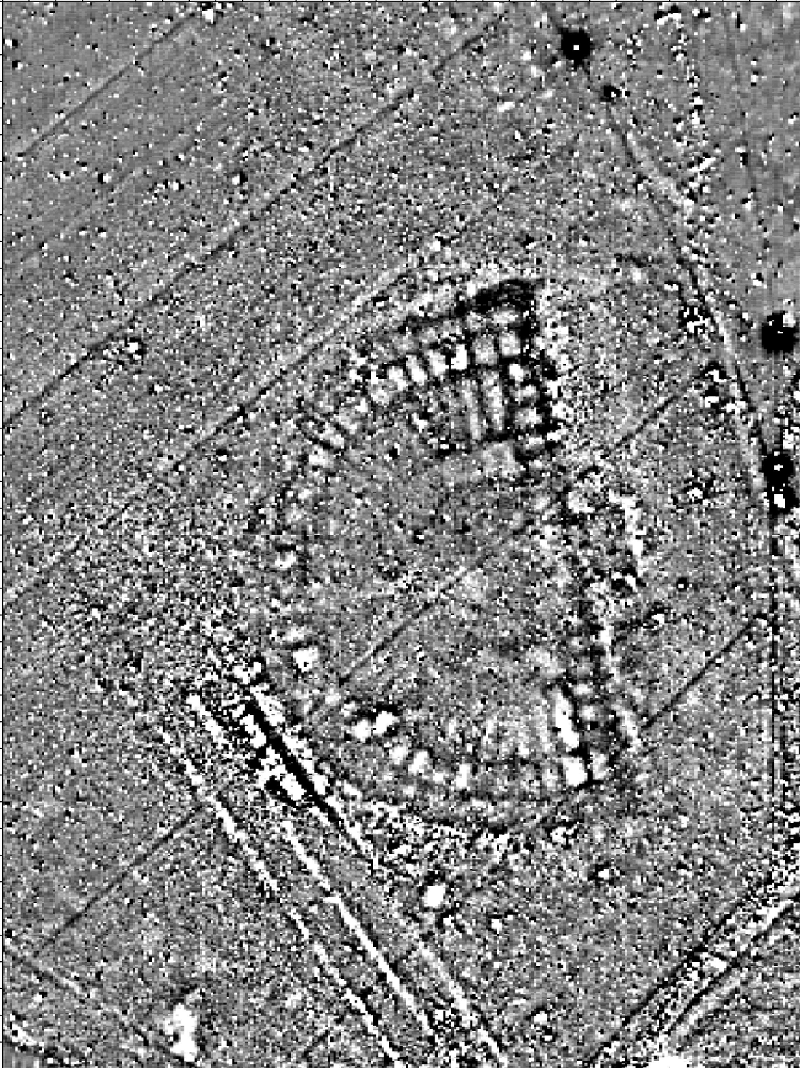
\includegraphics[width=5cm]{filter_input.png}
		\caption{Exemple d'image bruitée}. 
		\label{fig:FilterInput}
	\end{figure}
	Nous avons pour cela commencé par appliquer les techniques classiques de réduction de bruit : 
	\begin{itemize}
		\item Flou gaussien
		\item Filtres coupe-bande plus complexes (approche fréquentielle)
		\item Dilatation/Érosion
	\end{itemize}
	\newpage
	\paragraph{\textbf{Flou gaussien}}
	La manière la plus classique d'atténuer le bruit d'une image est le flou gaussien. Cette technique consiste à remplacer chaque pixel par la moyenne des ses voisins, avec une distance paramétrable.
	\begin{figure}[H]
		\centering
		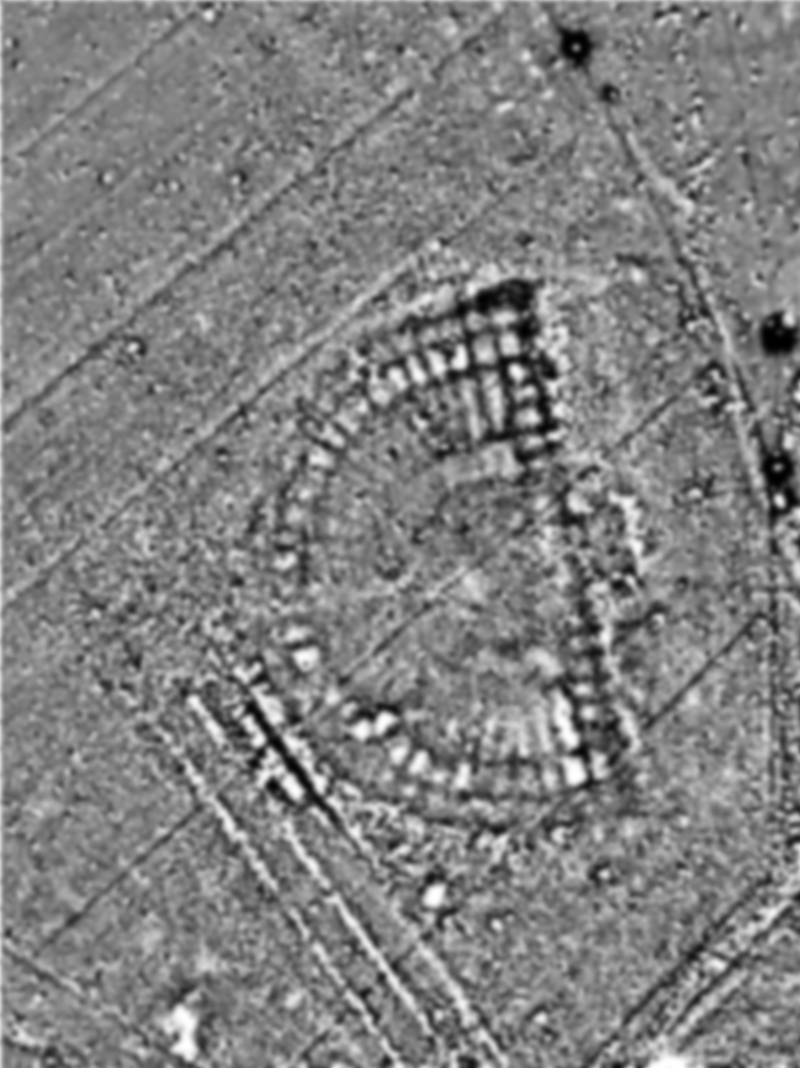
\includegraphics[width=6cm]{filter_gaussian.png}
		\caption{Image traitée avec un flou gaussien de 15 pixels}. 
		\label{fig:FilterGaussian}
	\end{figure}

	\newpage
	\paragraph{\textbf{Approche fréquentielle}}
	Ici, l'idée est d'appliquer le filtre sur directement sur la transformée de Fourier, affin de pouvoir choisir précisément les fréquences que l'on souhaite conserver ou supprimer.
	L'approche la plus concluante à été d'appliquer un passe-bande pour supprimer les hautes fréquences (qui contiennent le bruit), ainsi que les basses fréquences pour augmenter le contraste.
	\begin{figure}[H]
		\centering
		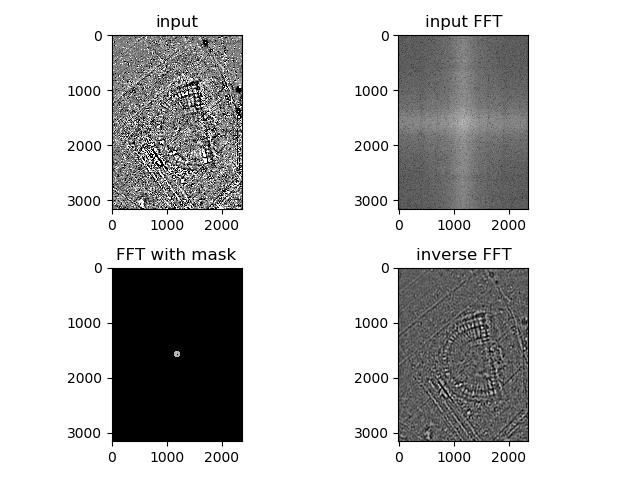
\includegraphics[width=\linewidth]{filter_fft.png}
		\caption{Différentes étapes du traitement}. 
		\label{fig:FilterFFT}
	\end{figure}
	On voit sur la figure \ref{fig:FilterFFT} le traitement séquentiel de l'image (de gauche à droite, puis de haut en bas) : on calcule la FFT, on applique un masque (le coupe-bande), puis on applique la FFT inverse. \\
	Cette approche peut donner des résultats intéressants, mais le problème est que la bande de fréquence à garder dépend des images. On perd donc de vue l'objectif initial, : l'automatisation.

	\newpage
	\paragraph{\textbf{Dilatation/Érosion}}
	La dilatation et l'érosion sont des traitements qui travaillent sur la morphologie de l'image.
	La dilatation "dilate" les formes : elle augmente la superficie des structures.
	À l'inverse, l'érosion réduit la superficie des structures, elle "érode" les bords.
	\begin{figure}[H]
		\centering
		\begin{subfigure}[b]{0.3\linewidth}
			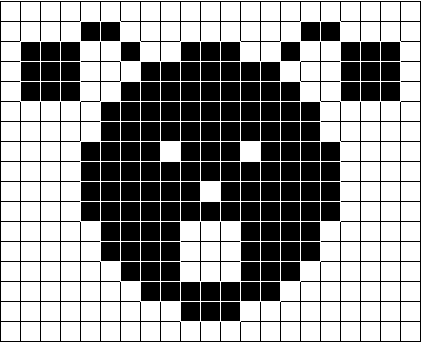
\includegraphics[width=\linewidth]{filter_dilate-erode_ex-base.png}
			\caption{Image originelle}
		\end{subfigure}
		\begin{subfigure}[b]{0.3\linewidth}
			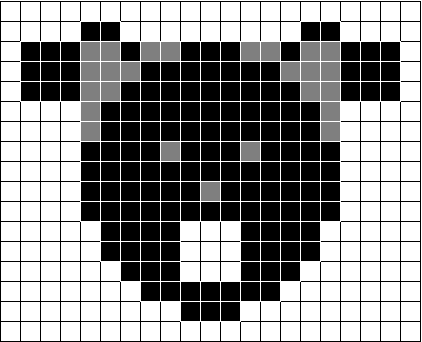
\includegraphics[width=\linewidth]{filter_dilate-erode_ex-dilate.png}
			\caption{Dilatation}
		\end{subfigure}
		\begin{subfigure}[b]{0.3\linewidth}
			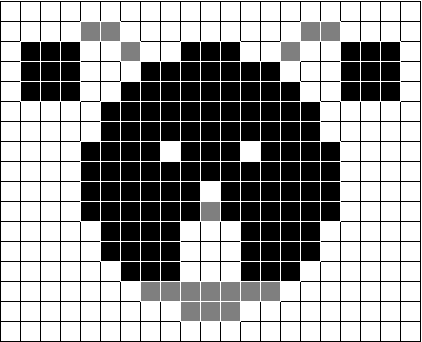
\includegraphics[width=\linewidth]{filter_dilate-erode_ex-erode.png}
			\caption{Érosion}
		\end{subfigure}
		\caption{Exemple de dilatation et d'érosion sur une image simple}. 
		\label{fig:FilterDilateErodeEx}
	\end{figure}
	L'érosion permet donc de supprimer les petites formes, nous pouvons donc l'utiliser pour effacer notre bruit.
	Pour compenser l'effet de l'érosion sur le reste de l'image, nous appliquons aussi une dilatation : le bruit est complètement effacé, et le reste est restauré par la dilatation.

	\begin{figure}[H]
		\centering
		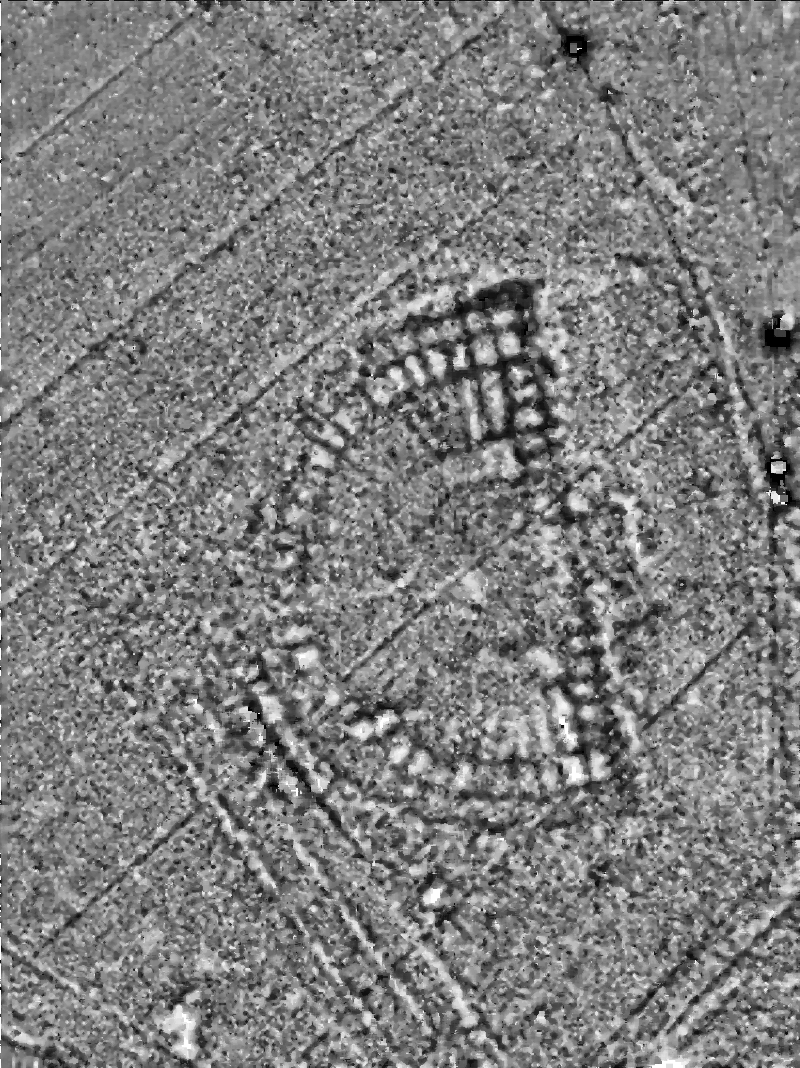
\includegraphics[width=6cm]{filter_dilate-erode.png}
		\caption{Image traitée par 2 érosions suivies de 2 dilatations}. 
		\label{fig:FilterDilateErode}
	\end{figure}

	\newpage
	\paragraph{\textbf{Conclusion}}
	Les techniques classiques de réduction de bruit dans une images semblent donner des résultats prometteurs : visuellement, l'image est plus lisible. Le résultat n'est cependant pas satisfaisant car, d'une part, le bruit reste présent, mais d'autre part -- et c'est le plus important -- le bruit n'est pas suffisamment effacé pour une détection de contours, comme nous allons le voir juste après.

	\newpage

	\subsubsection{Algorithmes de détections de bords}
	Nous avons débuté par l'utilisation de l'opérateur de Sobel\cite{SobelOp}. Cette technique produit des images en noir et blanc ou les bords ont une valeur de blanc élevé. Un bord est défini comme un endroit de l'image ou la magnitude de son gradient est élevé. Cette technique est très couramment utilise en \textit{Computer Vision} et il est déjà implémenté dans la librairie openCV en Python. Son fonctionnement est décrit en plus de détails ci-dessous: 
		\paragraph{\textbf{Recherche du gradient d'intensité de l'image}}
				On applique un kernel de Sobel: il s'agit simplement de deux matrices 3x3 permettant de calculer la dérivé première verticale et horizontale par convolution. Ces deux matrices sont:
				\\ \[G_x = \begin{bmatrix}  +1  & 0 & -1 \\ +2 & 0 & -2  \\ +1 &  0 & -1\end{bmatrix} 
					G_y = \begin{bmatrix} +1 & +2 & +1  \\  0 & 0 &  0  \\ -1 & -2 & -1\end{bmatrix}\]
						A chaque point de l'image on détermine la magnitude de ce gradient par la formule
					\[\nabla(G) = \sqrt{G_x^2 + G_y^2}\]
	\paragraph{\textbf{Création d'une image des bords}}
	Une fois cet opération réalisée, il nous suffit d'associer la valeur du gradient a une valeur de gris. Une grande magnitude du gradient, indiquant que le pixel orignal appartenait a un bord donnera un pixel blanc, tandis qu'une faible intensité donnera un pixel noir.
	Sur des images "propres" on obtient ce genre de résultats:
	\begin{figure}[H]
		\centering
		\begin{subfigure}[]{0.4\linewidth}
			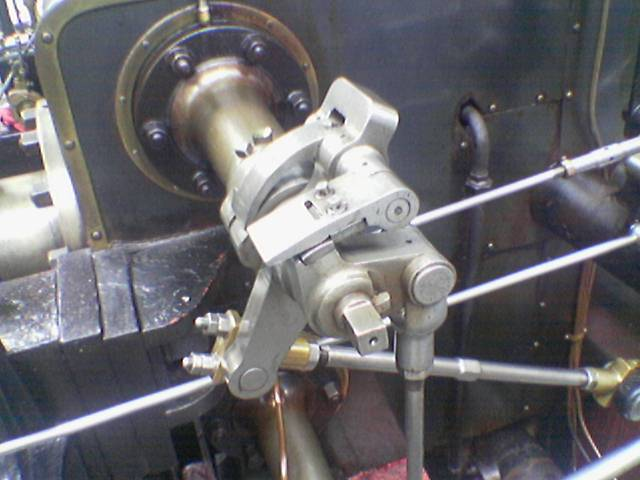
\includegraphics[width=\linewidth]{ValveOriginal.png}
			\caption{Image originelle}
		\end{subfigure}
		\begin{subfigure}[]{0.4\linewidth}
			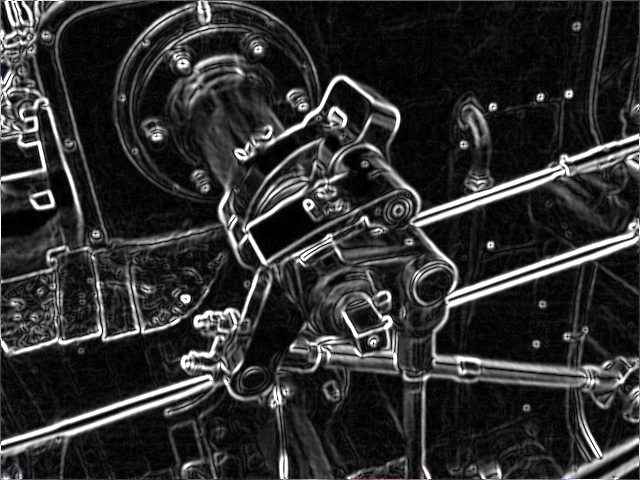
\includegraphics[width=\linewidth]{ValveSobel.png}
			\caption{Image traite avec Sobel}
		\end{subfigure}
		\caption{Comparaison d'une image sans traitement avec celle traite avec Sobel, de Wikipédia \cite{WikiCannyOriginal}\cite{WikiSobel}}. 
		\label{fig:SobelGood}
	\end{figure}
	On observe que les détails de l'image disparaissent, et que les bords, c'est a dire les endroits ou la magnitude du gradient de l'image sont important sont visible par des nuances de gris.
	\newpage
	Lorsque l'on applique l'opérateur Sobel sur nos images, nous obtenons, dans les meilleurs des cas, ces résultats:
	\begin{figure}[H]
		\centering
		\begin{subfigure}[]{0.4\linewidth}
			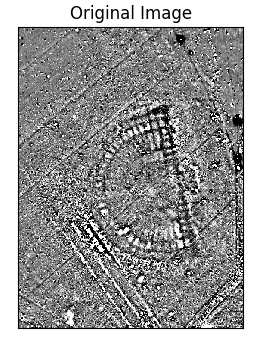
\includegraphics[width=\linewidth]{Sobel1b.png}
			\caption{Image originelle}
		\end{subfigure}
		\begin{subfigure}[]{0.4\linewidth}
			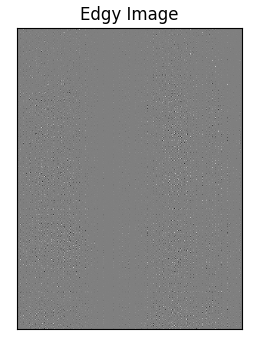
\includegraphics[width=\linewidth]{Sobel1a.png}
			\caption{Image traite avec Sobel}
			
		\end{subfigure}
		\caption{Traitement du relevé magnéto-métrique de l'amphithéâtre de Tarquimpol (Moselle), avec l'opérateur Sobel}
		\label{fig:OurSobel}
	\end{figure}

	Sur nos images, les résultats obtenus ne sont pas très pertinent. Le bruit est trop prévalent, et les bords des objets que nous cherchons a détecter sont trop faibles pour que l'opérateur de Sobel puisse donne des résultats intéressant.

	Nous avons ensuite décidé d'utiliser un autre algorithme, celui de Canny \cite{CannyOp}. L'algorithme de Canny reprend les matrices de Sobel, et applique quelques opérations supplémentaire pour obtenir des bords mieux défini. Les détails de l'algorithme sont décrit ci-dessous
	\begin{enumerate}
		\item \textbf{Réduction du bruit:}\\
			\indent On applique un filtre Gaussien 5x5 pour réduire le bruit présent dans l'image
		\item \textbf{Recherche du gradient d'intensité de l'image:}\\  
			\indent On applique ensuite un kernel de Sobel sur l'image "lisse" dans les directions verticales et horizontales afin d'obtenir les dérivés premières dans
			la direction verticale $G_x$ et horizontales $G_y$. Ce procédé est identique a celui décrit plus haut.

		\item \textbf{Suppression des non maximums locaux}\\
			\indent Une fois les gradients obtenus, on analyse tout les pixels de l'image, et on détermine si le pixel est un maximum local dans la
			direction du gradient. \\
			Si oui, c'est un bord et sa valeur est garde pour la prochaine étape, sinon, elle est mise a 0. On obtient une image binaire, avec que des bords

		\newpage

		\item \textbf{Seuil d'Hysterisis} \\
			\indent On utilise deux seuils, $minVal$ et $maxVal$. Tout les bords ayant une intensité de gradient supérieur a $maxVal$ est forcement un
			bord, ceux en dessous de $minVal$ sont forcement des non-bords, et sont donc abandonne. Les bords qui sont entre ces deux seuil sont classe
			"bords" ou "non-bords" selon leur connectivité. Si ils sont connecte a des pixels qui sont des forcement des bords, alors ce sont des bords,
			sinon, ils sont aussi abandonne.\\

	\end{enumerate}
	Encore une fois cet algorithme était déjà disponible dans la librairie d'analyse de d'image PythonCV2, nous n'avons pas eu a l'implémenter, et nous avons bénéficié de quelques optimisations rendant l'exécution plus rapide.
	Avec une image "propre", on obtient ce genre d'image:
	\begin{figure}[H] %%NE PAS OUBLIER DE LINK L'AUTEUR : By Simpsons contributor, CC BY-SA 3.0, https://commons.wikimedia.org/w/index.php?curid=8904364
		\centering
		\begin{subfigure}[]{0.4\linewidth}%CORIGER LA POSITION DES FIGURES
			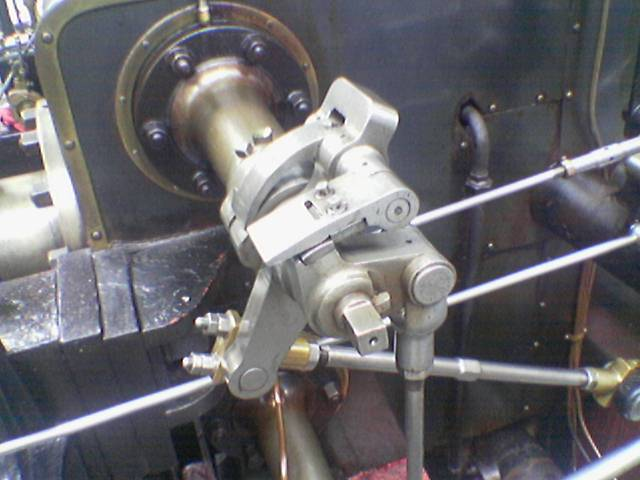
\includegraphics[width=\linewidth]{ValveOriginal.png}
			\caption{Image originelle}
		\end{subfigure}
		\begin{subfigure}[]{0.4\linewidth}
			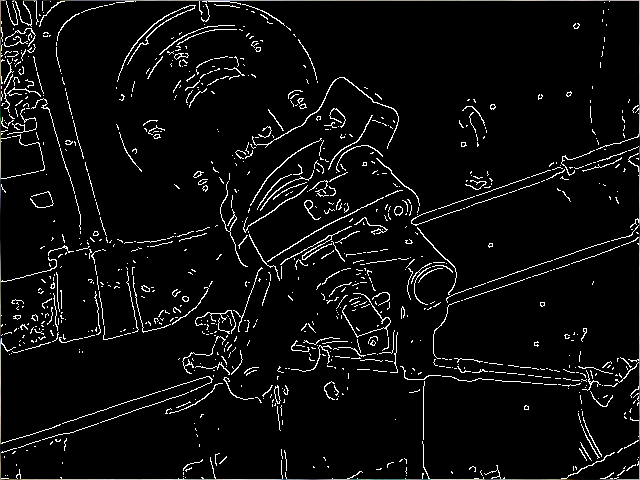
\includegraphics[width=\linewidth]{ValveCanny.png}
			\caption{Image traite avec Canny}
		\end{subfigure}
		\caption{Comparaison d'une image sans traitement avec celle traite avec Canny, de Wikipedia \cite{WikiCannyOriginal}\cite{WikiCanny}}. 
		\label{fig:cannyGood}
	\end{figure}
	On observe que les bords sont bien plus défini, et propre par rapport a ceux obtenu avec l'opérateur Sobel. Mieux, les bords "majeurs", sont préservé, alors que les bords "mineurs" disparaissent. Cela est du aux deux dernières étapes de l'algorithme de Canny.
	Lorsque l'on applique Canny a nos images, nous obtenons ceci:
	\begin{figure}[H]
		\centering
		\begin{subfigure}[]{0.4\linewidth}
			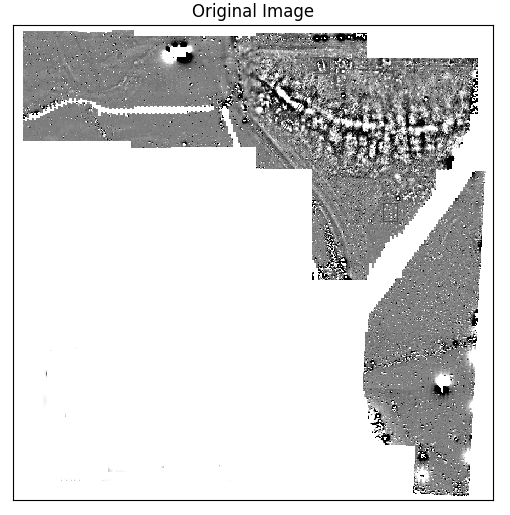
\includegraphics[width=\linewidth]{Canny1a.png}
			\caption{Image originelle}
		\end{subfigure}
		\begin{subfigure}[]{0.4\linewidth}
			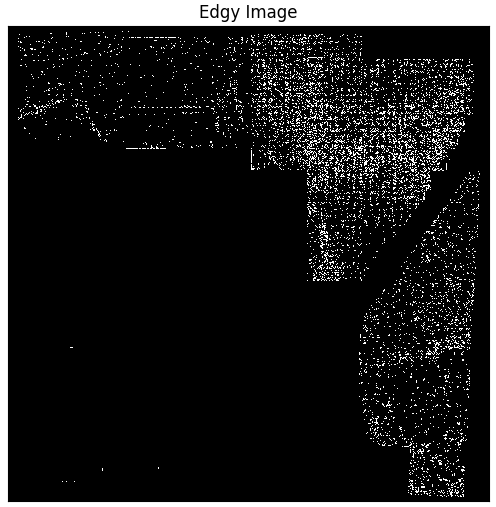
\includegraphics[width=\linewidth]{Canny1b.png}
			\caption{Image traite avec Canny}
		\end{subfigure}
		\label{fig:OurCanny}
	\end{figure}

	Même si il y a une amélioration certaine par rapport a Sobel, l'algorithme ne parvient toujours pas a trouver les contours des objets d'intérêt, encore une fois a cause du a la grande quantité de bruit que l'on trouve dans l'image. Cependant  on observe une densité de points plus élevé aux niveau des endroits d'intérêts, comme ici, et une densité faible dans les zones ou on ne trouve ni objets ni bruit.
	%Rajouter comparaison Canny Sobel sur Amphi.png
	\begin{figure}[H]
		\centering
		\begin{subfigure}[]{0.4\linewidth}
			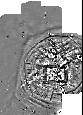
\includegraphics[width=\linewidth]{CANNY_ExempleDetailsA.png}
			\caption{Image originelle}
		\end{subfigure}
		\begin{subfigure}[]{0.4\linewidth}
			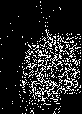
\includegraphics[width=\linewidth]{CANNY_ExempleDetailsB.png}
			\caption{Image traite avec Canny}
		\end{subfigure}
		\caption{Comparaison de détails entre une image sans traitement avec peu de bruit, et l'image traite avec Canny. Même si les bords ne sont pas détecté correctement, les lieux d'intérêt de l'image (la forme circulaire) ont très visiblement une haute densité de points.}
		\label{fig:CannyDetails}
	\end{figure}

	\subsubsection{Problèmes rencontres}
	De toute évidence, nous avions atteint un obstacle: le bruit. Celui ci était présent sur toutes les images, au point d'empêcher toute tentative d'analyse classique de signal. La magnétométrie est très sensible aux objets métalliques, et dans la région ou ont été fait les relevés, de nombreux objets métalliques contemporains sont présent dans le terrain, notamment a cause des combats de la 2\textsuperscript{ème} guerre mondiale, mais aussi a cause des labours, et du déchets métallique produit par l'occupation humaines de ces terrains.\\
	Une analyse classique ne suffisait donc pas, et le développement de méthodes de filtrage et de détection de bords étant capable de traiter des images aussi bruite est hors de notre porte. Notre attention devait donc se porter sur la résolution d'un problème, annexe a celui qui nous intéressait, mais dont les techniques développé par sa résolution pouvait nous aider dans notre objectifs principal.

\newpage
\section{Développement d'une nouvelle méthodologie}
	\subsection{Détection d'objets métalliques par réseaux neuronaux}
	Comme dit plus haut, les techniques classiques utilise dans l'analyse d'image sont inapplicables dans notre cas, du notamment au haut niveau de bruit présent dans les images a traites. Cependant, il est évidents que ce bruit n'est pas identique aux objets que nous cherchons, car sinon, les archéologues ne pourrait pas analyser ces images. Pour mieux diriger nos recherches nous avons choisi de détecter un type particulier de signaux, ceux provenant d'objet métalliques. Les réseaux de convolution sont très adapte a cette taches; car ils filtrent l'image et développent eux même les règles qui définissent l'objet ainsi que leur filtres. Ils permettent de détecter des motifs dans des parties de l'image, et non plus sur des pixels individuels, comme était le cas avec le filtrage ou la détection de bords. De plus, nous construisons un réseau n'apprenant a détecter qu'une seule classe d'objet, ce qui rendra l'apprentissage plus rapide. Si nous réussissons a détecter ces objets métalliques, nous pouvons alors:
	\begin{enumerate}
		\item "Nettoyer" les cartes de ces objets, qui ont tendance a rendre difficile la lecture, en appliquant un flou gaussien par exemple
		\item Utiliser le même réseau dans la détection de plus d'objet, en transférant l'apprentissage déjà fait sur un plus grand nombre de classe
	\end{enumerate}

	\subsubsection{Caractérisation}
	Les dipôles proviennent des objets métalliques contemporains, et se caractérisent par un pôle positif très fort au niveau de l'objet, suivi d'un halo circulaire négatif, dont le diamètre est approximativement 2 fois celui de l'objet. On peut voir sur la figure \ref{fig:DipoleExample} que les anomalies se ressemblent beaucoup, et son très présentes sur virtuellement toutes les cartes. De plus elles sont assez grandes pour être immédiatement reconnu sur nos relevés, ce qui simplifie la tache d'annotation des exemples a apprendre. 

Un aspect intéressant de ce problème est, bien que si les dipôles produit par des objets métalliques contemporains sont généralement considère comme du bruit, ce n'est parce qu'ils \textit{ne font pas partie de la période recherche}. En d'autre terme, un objet métallique récent est un objet archéologique comme les autres: il provient d'une certaine période historique, a une ou plusieurs techniques de fabrication qui lui sont propre, provient d'un certains lieu... Dans certaines circonstance de recherche, en particulier lorsque le site et les objets est date de la protohistoire, des objets datant de l'occupation romaine sont vu comme du bruit. C'est le cas avec le site de Marsal, ou une occupation romaine a eu pour conséquence des rejets de déchets datant de l'ère romaine, comme des tuiles, qui provoque du "bruit" sur nos cartes. En somme, il ne faut pas voir notre approche comme une recherche de "bruit", mais simplement comme un changement d'objet d'intérêt. Nous en choisissons un distinct, commun, et donc plus facile a étudier.
	%RAJOUTER IMAGE DIPOLE REEL
	%RAJOUTER PLOT3D DIPOLE
	\begin{figure}[H]
		\centering
		\begin{subfigure}[b]{0.3\linewidth}
			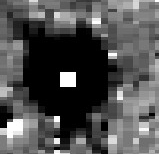
\includegraphics[width=\linewidth]{DipoleExemple1.png}
		\end{subfigure}
		\begin{subfigure}[b]{0.3\linewidth}
			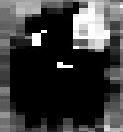
\includegraphics[width=\linewidth]{DipoleExemple2.png}
		\end{subfigure}
		\begin{subfigure}[b]{0.3\linewidth}
			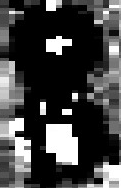
\includegraphics[width=\linewidth]{DipoleExemple3.png}
		\end{subfigure}

		\caption{Quelques exemples de dipôles, récupéré sur plusieurs relevés différents. On peut observer leur similitudes, tant par leur formes que par leur tailles}
		\label{fig:DipoleExample}
	\end{figure}

	\subsubsection{Explication de l'approche}
	Les réseaux de convolution sont une innovation récente dans le champs de l'apprentissage automatique. Le premier exemple d'un réseau de convolution moderne provient de Yann Le Cun \cite{lecun-01a} en 1998. En 2012, les réseaux de convolution réapparaitront avec AlexNet \cite{NIPS2012_4824}, et restent aujourd'hui sur le devant de la scène de l'apprentissage automatique. 
	Les réseaux de convolutions, que nous appellerons CNNs (Convolutionnal Neural Network) se composent de 2 parties
	%EXPLICATION CNNS
	\newpage
	\subsubsection{Problèmes initiaux}
	Un des difficultés principale attache a ce projet est le petit nombre initial d'exemples. En tout, nous possédons 41 Relevés géophysique. De toute évidence, une telle quantité de données ne suffirait pas a entrainer un modèle : les bases de données modernes, en particulier celle d'images se compose de plusieurs centaine de milliers d'exemples; par exemple imageNet comporte plus de 14 Millions d'exemple (\url{http://image-net.org/about-stats}). Nous devons alors trouver des méthodes permettant d'augmenter artificiellement le nombre d'exemple en prenant garde que ces exemples crée synthétiquement représente toujours bien la réalité. De plus nous ne possédions aucune compétence en terme d'apprentissage automatique, et nous allions devoir tout apprendre. 
	\subsubsection{Solutions}
	\textbf{Génération d'exemple}:\\
	Classifier a la main tout les exemples nécessaires a l'entrainement du réseau était une tache surhumaine. Par soucis d'efficacité, nous avons décidé de construire nous même
	nos exemples, et des les utiliser en combinaison avec des exemples provenant des images, et classifie a la main.
	Pour avoir une meilleure chance de créer un bruit proche de la réalité, nous avons utilise 2 approches différentes:
	\begin{itemize}
		\item Une approche informatique
		\item Une approche mathématique
	\end{itemize}
	L'approche informatique consiste a créer 2 cercles, de tailles variables,un noir et un blanc, ayant la même origine. Ces cercles sont imprime sur une \textit{backplate} grise avec du bruit génère aléatoirement. Afin d'améliorer le résultat, du bruit est ajoute aux cercles, augmentant particulièrement aux bords de ceux ci.

	Nous avons génère une fonction mathématique se rapprochant de celle d'un dipôle.\\
	Il s'agit d'une fonction sinusoïdale amortie exponentiellement modifie pour que sont domaine soit $\mathbb{R}^2 \to \mathbb{R}$:
	\[f(x,y) = A.e^{-\lambda . \sqrt{(x+i)^2+(y+j)^2}}.\cos(\omega . \sqrt{(x+i)^2+(y+j)^2} + \phi)\]
	Avec:\\
	\indent $A$ l'amplitude initiale, choisie aléatoirement entre 200 et 255\\
	\indent$\lambda$ coefficient d'amortissement\\
	\indent$\omega$ vitesse angulaire\\
	\indent$\phi$ angle de phase a l'origine\\
	\indent$i,j$ décalage horizontal et vertical, respectivement, par rapport a l'origine

	Avec la génération aléatoire des paramètres de cette fonction, nous pouvons obtenir une grande variété d'exemple qui ressemble aux dipôles retrouves dans nos cartes. 
	%TODO: Rajouter exemple 3D Dipole Reel vs Dipole Genere
	%TODO: Source image : Document PZP (Lieu)
	\textbf{Traitement des images}:\\%Rajouter Schema explicatif
	\indent Afin d'obtenir une meilleure qualité d'exemples nous avons utilise ceux provenant de nos données originelle. Nous avons d'abord découpe chacune des images en carre de taille 96*96 pixels; en décalant le carre de 48 pixels verticalement et horizontalement a chaque fois, nous pouvons obtenir encore plus d'exemples. En décalant la fenêtre qui obtient le carre de 48 pixels, on obtient un également un meilleur recouvrement des pixels.

	
\begin{figure}[H]
		\centering
		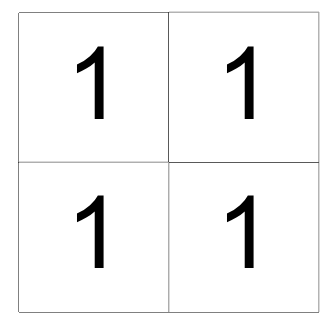
\includegraphics[width=\linewidth]{ExempleCarre.png}
		\caption{Représentation du nombre de fois ou une zone a été recouverte, ici avec un décalage de la taille du carre. Chaque zone est n'est couverte que par un seul carre}. 
		\label{fig:ExempleCarre}
\end{figure}

Les relevés dont nous disposons n'ont pas tous une forme rectangulaire. En effet il s'agit de plusieurs zones rectangulaire ou des relevés ont été fait, avec des zones blanches ou il n'y pas de relevés. Ces zones sans relevés nous sont inutile. Pour ne pas avoir de carre sans relevés, nous avons colore les zones blanches en vert (voir la figure \cite{ReleveColore} pour un exemple). Lors du découpage nous vérifions si notre image contient du vert (Notre vert est particulier car il contient un peu de rouge. Il s'agissait initialement d'une erreur). Si le carre contient du vert, cela veut dire qu'une partie, ou la totalité, du carre est une zone sans relevés.

\begin{figure}[H]
		\centering
		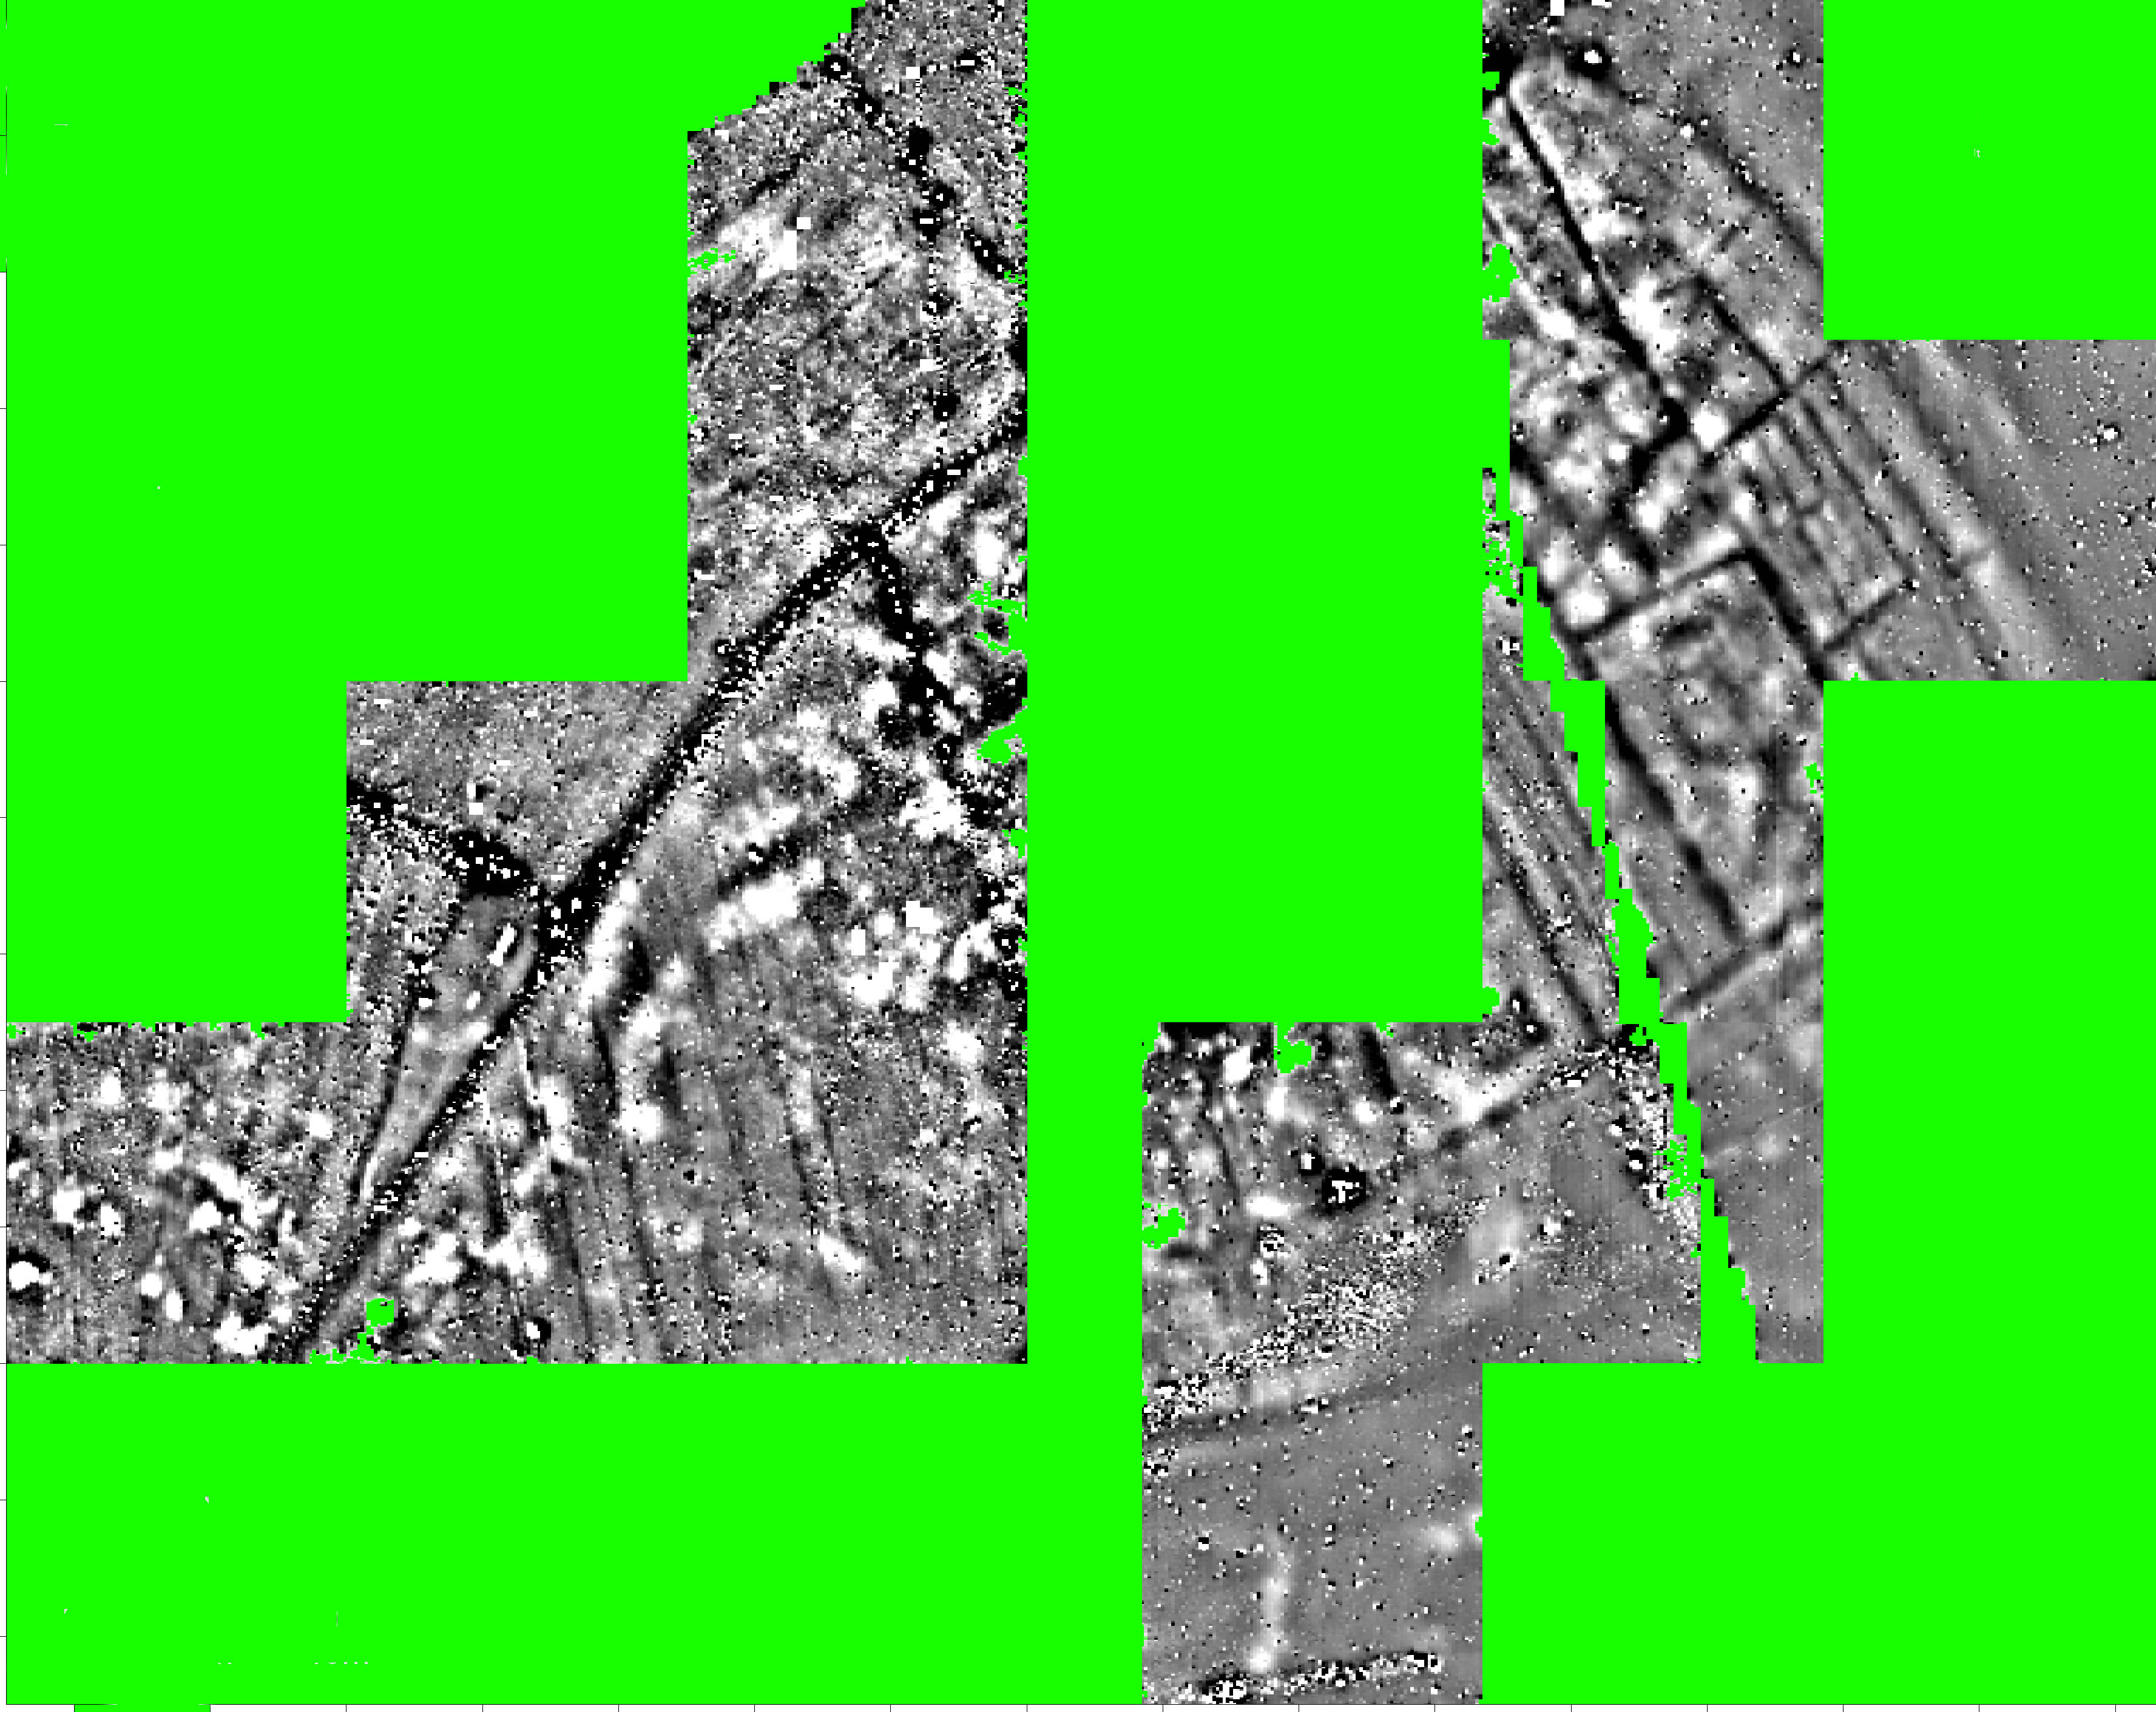
\includegraphics[width=6cm]{ExemplePretraitement.jpg}
		\caption{Retraitement d'une carte avec remplacement des zones sans relevés blanche par du vert}. 
		\label{fig:ReleveColore}
	\end{figure}

Au final, nous avons pu obtenir plus de 51000 carres, grâce au fait que les images était très grande (souvent plus de 2000*2000 pixels). Nous avons ensuite, a la main, trouve tous les carres contenant un dipôles, ce qui nous donne 413 images de dipôles. Ces images, provenant du monde réelle sont très variée, que ce soit par leur taille, leur position dans l'image ou encore leur nombre.

	Cependant, 400 images n'est toujours pas suffisant pour entrainer un réseau. Pour enrichir notre datasse nous avons décidé d'appliquer quelques transformations sur chacune des images. A l'heure ou nous écrivons ces lignes, nous avons implémenté les transformations suivantes :
	\begin{enumerate}
		\item Rotation de l'image sur l'axe x %Schema pour chacun de ces transfo
		\item Rotation de l'image sur l'axe y 
		\item Ajout de bruit
	\end{enumerate}
	
	\textbf{Implémentation Réseau Neuronal}\\
	\indent Nous avons implémenté un réseau neuronal classique s'entrainant sur des exemples générés. Le réseau reprends l'architecture de l'exemple de TensorFlow pour la classification de chiffres manuscrit avec une modification du nombre d'entrée pour s'adapter a la taille des exemples générés. Lors de l'entrainement, on a pu observer une très rapide maximisation du taux de détection, arrivant a un taux de réussite de 100\% sur les exemples de test en 4 époques. Nous avons ensuite tente d'appliquer ce réseau sur une carte, dans l'espoir de créer une \textit{heatmap} d'activation du réseau. Malheureusement, ce réseau possédait un taux d'erreur très élevé sur les exemples réels. Nous ne possédions pas le temps d'implémenter un réseau neuronal de convolution, et les résultats obtenu avec le réseau neuronal "classique" nous indiquait qu'utiliser seul des exemples génères ne suffirait pas pour obtenir un bon taux de détection sur les données réelles. Nous avons donc préférée utiliser notre temps restant a construire une meilleure base d'exemple en mixant données réelle et données générée, pour obtenir non seulement une meilleure variance, mais un \textit{dataset} plus proche de la réalité.
\newpage
\section{Conclusion}
	\subsection{Bilan Provisoire} %Changer le nom ?
	Ce semestre fut riche en travail et en résultat. Nous avons énormément appris sur le travail d'analyse de données, le nettoyage de \textit{dataset}, les réseaux d'apprentissage automatique, ainsi que des techniques d'analyse d'image. Le travail de mise en place de système d'apprentissage automatique est un travail long et délicat; d'autant plus que nous possédons un corpus de données réduit. Malgré tout nous, nous sommes optimiste sur le déroulement de ce projet. Le travail de ce premier semestre ne fut pas que lecture d'article académique: nous avons pu observe que les techniques traditionnelles d'analyse d'image ne fonctionne pas avec nos données, nous avons crée un corpus de données annote de plus de 50 000 images, et pose les bases pour l'implémentation d'un réseau de convolution.
	\subsection{Implémentation d'un réseau de convolution}
	La prochaine étape est évidement l'implémentation d'un réseau de convolution, apprenant sur le \textit{dataset}. La partie la plus chronophage, celle de préparer la base de données étant déjà accompli, cette tache ne prendra que peu de temps. 
	\subsection{Choix de la direction de recherche}
	Nous devons maintenant décider de la direction de nos recherches pour le Semestre 2. L'implémentation d'un réseau de convolution, et l'analyse des résultats obtenus, nous permettre de faire une décision sur le choix des objets a analyser. Si le réseau donne une précision en déca de nos attentes, nous continuerons notre travail sur l'analyse d'objet métalliques. Si nous obtenons une précision acceptable alors nous pouvons alors étendre celui ci a l'étude d'autres objets archéologiques dont la définition en tant que structure dans une image est plus complexe, comme des tombes, des routes, etc. 

	Nous désirons également pouvoir travailler avec d'autres types de relevés, a utiliser en conjonction avec nos cartes magnéto-métrique, comme par exemple le LIDAR, ou le radar de sol. Cependant obtenir ces relevés n'est pas une tache aise, d'autant plus qu'ils couvrent généralement des zones différentes de celles couvertes par la magnétométrie.

	Ensuite, nous voudrions encore enrichir notre corpus de données : des avances récentes ont été faite a ce sujet \cite{Transfo}, et il serait intéressant de pouvoir les utiliser. Finalement, nous nous posons la question de rendre ce corpus public, après autorisation auprès des propriétaires, bien sur. Des corpus sur les objets archéologiques dans ce contexte sont virtuellement inexistants, et serait un ajout pertinent. 
\newpage
\section{Annexes}




\subsection{Scripts}
\subsubsection{Script appliquant Canny sur tous nos relevés}
\begin{verbatim}
#canny.py
import numpy as np
import cv2

from matplotlib import pyplot as plt
from os import listdir
from os.path import isfile, join




files = [ f for f in listdir("../Data/") if isfile(join("../Data/",f))]

for image in files:
    print "Analysing "+image
    img = cv2.imread("../Data/"+image , 0)
    edge = cv2.Canny(img,100,200)

    plt.subplot(121), plt.imshow(img, cmap='gray')
    plt.title('Original Image'), plt.xticks([]), plt.yticks([])

    plt.subplot(122), plt.imshow(edge, cmap='gray')
    plt.title('Edgy Image'), plt.xticks([]), plt.yticks([])

    filename = "output/CANNY_"+image
    plt.savefig(filename)
\end{verbatim}

\subsubsection{Script decoupant nos relevés en carrés de 96x96}


\begin{spverbatim}
#CutImage.py

#Importation des librairies necessaire
from PIL import Image #Python Image Library

from os import listdir
from os.path import isfile, join

#On recupere les fichiers du repertoire PreparedData
files = [f for f in listdir("../Data/PreparedData/") if isfile(join("../Data/PreparedData/", f))]


n = 0

#Fonction pour verifier si un carre est en noir et blanc
def CheckGrayScale(img):
    img = img.convert('RGB')
    w,h = img.size

    #On itere a travers tous les pixels de l'image
    for i in range(w):
        for j in range(h):
            r,g,b = img.getpixel((i,j))
            if (r == 24 and g==255 and b==0):#Si le pixel contient notre vert alors on renvoie faux

                return False
    return True

for image in files:
    n += 1
    print "Analysing "+image+"[",n,"/",len(files),"]"

    img = Image.open("../Data/PreparedData/"+image)#On ouvre l'image

    width, height = img.size

    #On decoupe l'image en carre de 96*96 avec un recouvrement de moitie

    StrideX=48 #Decallage horizontal du carre
    StrideY=48 #Decallage vertical du carre
    numSquareLine = width/StrideX #Nombre de carre sur une ligne
    numSquareCol = height/StrideY #Nombre de carre sur une colonne

    print "Width = ", width, "Height =  ", height
    print "Num Squares Line =",numSquareLine,"Num Square Col =", numSquareLine
    print "StrideX=", StrideX, "StrideY=", StrideY
    print "\n"

    for i in range(numSquareCol): #On itere de 0 au nombre de carre dans une colonne
        for j in range(numSquareLine): #On itere de 0 au nombre de carre dans une ligne
            
	    #On decoupe l'image en un carre de 96*96, en decallant a chaque fois de 48 pixels horizontalement et verticalement
	    imgCropped = img.crop((j*StrideX, i*StrideY, 
	    j*StrideX+96, i*StrideY+96))

	    #On genere un filename avec les coordoones de l'image
            Filename = "PreparedData/"+image+"("+str(j*StrideX)
	    +","+str(i*StrideY)+")("+str(j*StrideX+96)+","+str(i*StrideY+96)+").png" 
            
	    imWidth, imHeight = imgCropped.size
            
	    #Si la taille de l'image est correcte ET si celle ci ne contient pas de vert, alors on enregistre
	    if (imWidth == 96 and imHeight == 96 and CheckGrayScale(imgCropped) == True):
                imgCropped.save(Filename)

\end{spverbatim}


\medskip
\newpage
\printbibliography
\end{document}
